\documentclass{article}

\usepackage{pdfpages}
\usepackage{graphicx}

\usepackage{float}

\usepackage{adjustbox}
\usepackage{hyperref}

\usepackage{biblatex}
\addbibresource{references.bib}

\graphicspath{ {./images/} }

\title{
    \vspace{-4.0cm}
    {\Huge Social Routing}\\[0.5cm]    
    \textsc{\Large Project and Seminar}\\[0.5cm]
    \textsc{\large ISEL - Instituto Superior de Engenharia de Lisboa}\\[0.5cm]
    \textsc{\large (Inglês?) Licenciatura em Engenharia Informática e de Computadores}\\[0.5cm]
}

\date{\today}
\author{   
    \begin{minipage}{0.4\textwidth}
        \begin{flushleft} \large
        \emph{Authors:}\\
        Baltasar Brito\\
        {\small email: baltasar.brito@gmail.com}\\
        {\small phone: 915953552}\\
        Bernardo Costa\\
        {\small email: bjmcosta97@gmail.com}\\
        {\small phone: 913897555}\\
        \end{flushleft}
    \end{minipage}
    ~
    \begin{minipage}{0.4\textwidth}
        \begin{flushright} \large
        \emph{Supervisor:} \\ 
        Pedro Félix\\
        {\small email: pedrofelix@cc.isel.ipl.pt}\\  
        \end{flushright}
    \end{minipage}\\[2cm]  
}

\begin{document}     
    
    \maketitle

    \newpage

    \tableofcontents

    \newpage

    \section{Introduction}

    \section{Background}
    trabalho relacionado, sistemas ou aplicações similares
    características dos dados

    \section{Specifications}
    requisitos, escolha de tecnologias, bibliotecas e plataformas

    \section{Project Structure}
        The project still follows the same System Structure that was established initially in the proposal, which has two major components and a 
        third exterior one, communicating with each other, separating concerns and business logic. The following figure illustrates the system's structure:
        
        \begin{figure}[h]            
            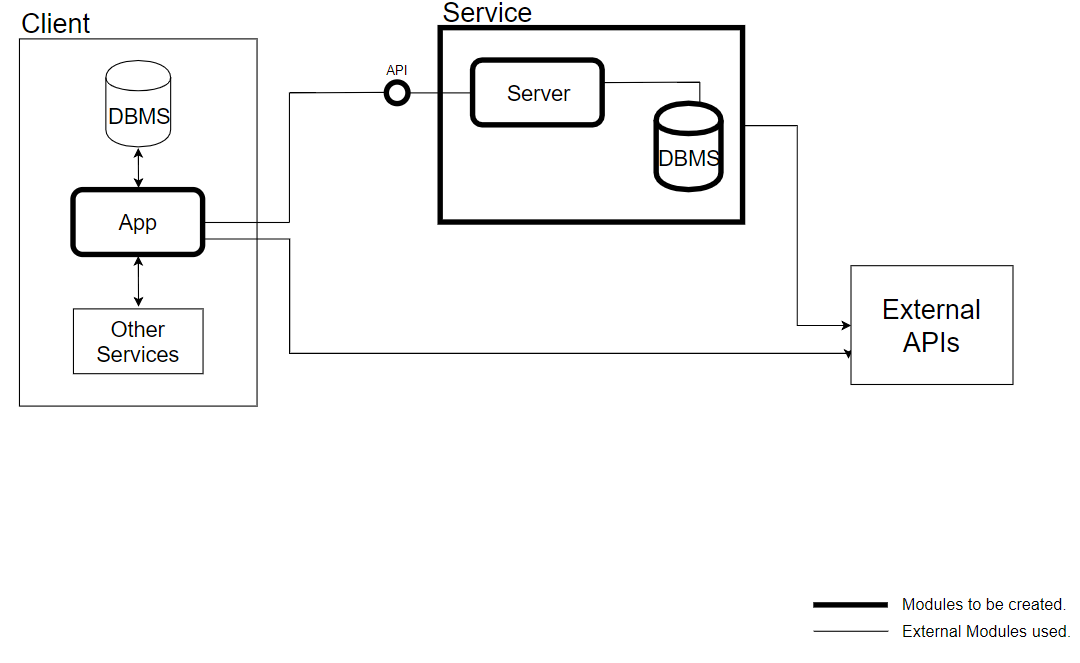
\includegraphics[width=\textwidth]{images/project-structure/system-structure.PNG}
            \caption{System structure.}
            \label{fig:systemstructure}
        \end{figure}  
    \newpage    

    \section{Implementation}
        breve introducao

        \subsection*{Social Routing Client Application}
        breve introducao
        imagem com estrutura interna
        explicacao de cada componente da estrutura interna

        \subsection*{Social Routing Service}
        breve introducao
        imagem com estrutura interna
        explicacao de cada componente da estrutura interna

    \section{Tests}
    
    \section{Timeline Evaluation}

    \section{Conclusion}

    \printbibliography

\end{document}